Zunächst wird die akustische Mikroskopie verwendet, um darstellen zu können, wie eine Zerstörung freie Untersuchung erfolgen kann, darüber hinaus werden nach Risse und Schaden untersucht und mögliche Darstellung bemerken zu können wie Luftblasen. Diese Untersuchung wird mit drei Proben durchgeführt.
Aufgabe bei den Proben ist auch die Ebenen zu wählen, die für eine solchen Untersuchung sinnvoll sind.  Potentielle
Defekte oder Fehler müssen dokumentiert und erläutert werden.


In diesem Experiment werden drei unterschiedliche Proben mit dem KSI V8 SAM untersucht, um innere Strukturen und Defekte zerstörungsfrei zu erkennen. Die Messung erfolgt im Reflexionsmodus, wobei Ultraschallwellen über ein Wasserbad eingekoppelt und reflektierte Signale ausgewertet werden.

Die erste Probe ist eine keramische DCB-Leiterplatte mit gesinterten Halbleitern, teils mit Bonddrähten kontaktiert (siehe Abbildung 3). Sie dient zur Einführung in die SAM-Bedienung und zur Darstellung verschiedener Materialübergänge in mehreren Ebenen.

Die zweite Probe besteht aus einem Kupfer-Leadframe, der auf ein keramisches Substrat geschweißt wurde (siehe Abbildung 4). Hier liegt der Fokus auf der Analyse der Schweißverbindungen und der Untersuchung möglicher Defekte durch Wahl geeigneter Scanebenen.

Die dritte Probe ist ein DoL-Leistungselektronikmodul ohne Bonddrähte (siehe Abbildung 5). Statt keramischer Isolation kommt eine organische Trägerfolie zum Einsatz. Die Ebenenwahl und Bewertung erfolgen selbstständig.

Alle Proben werden im Wasserbecken positioniert, wobei auf die Entfernung von Luftblasen geachtet wird. Die Steuerung erfolgt über den integrierten PC, und nach jeder Messung wird das Gerät in die Home-Position zurückgefahren.



Die Untersuchung erfolgt mit dem Scanning Acoustic Microscope KSI V8 \cite{2}, einem Hochleistungsgerät zur zerstörungsfreien Prüfung und Fehleranalyse in Bereichen wie der Mikroelektronik, Materialwissenschaft und Halbleiterfertigung. Das Gerät arbeitet im Frequenzbereich von 5MHz bis 400MHz, wodurch sich die Eindringtiefe und Auflösung flexibel an das zu untersuchende Material anpassen lassen. Mit einer Scangeschwindigkeit von bis zu 2m/s und einer Positionsgenauigkeit von 1m ermöglicht der KSI V8 eine präzise und gleichzeitig zeiteffiziente Analyse.

Das System bietet mehrere Scanmodi, die eine detaillierte Untersuchung unterschiedlicher Strukturen ermöglichen. Im sogenannten C-Scan-Modus wird eine zweidimensionale Darstellung einer definierten Fokusebene erzeugt, die sich besonders zur Erkennung von Hohlräumen und Rissen innerhalb einzelner Materialschichten eignet. Ergänzend dazu erlaubt der B-Scan die Darstellung eines Tiefenprofils, während der 3D-Scan durch die Kombination mehrerer Ebenen eine volumetrische Abbildung des Probenaufbaus liefert.


\begin{figure}[htbp]
    \centering
    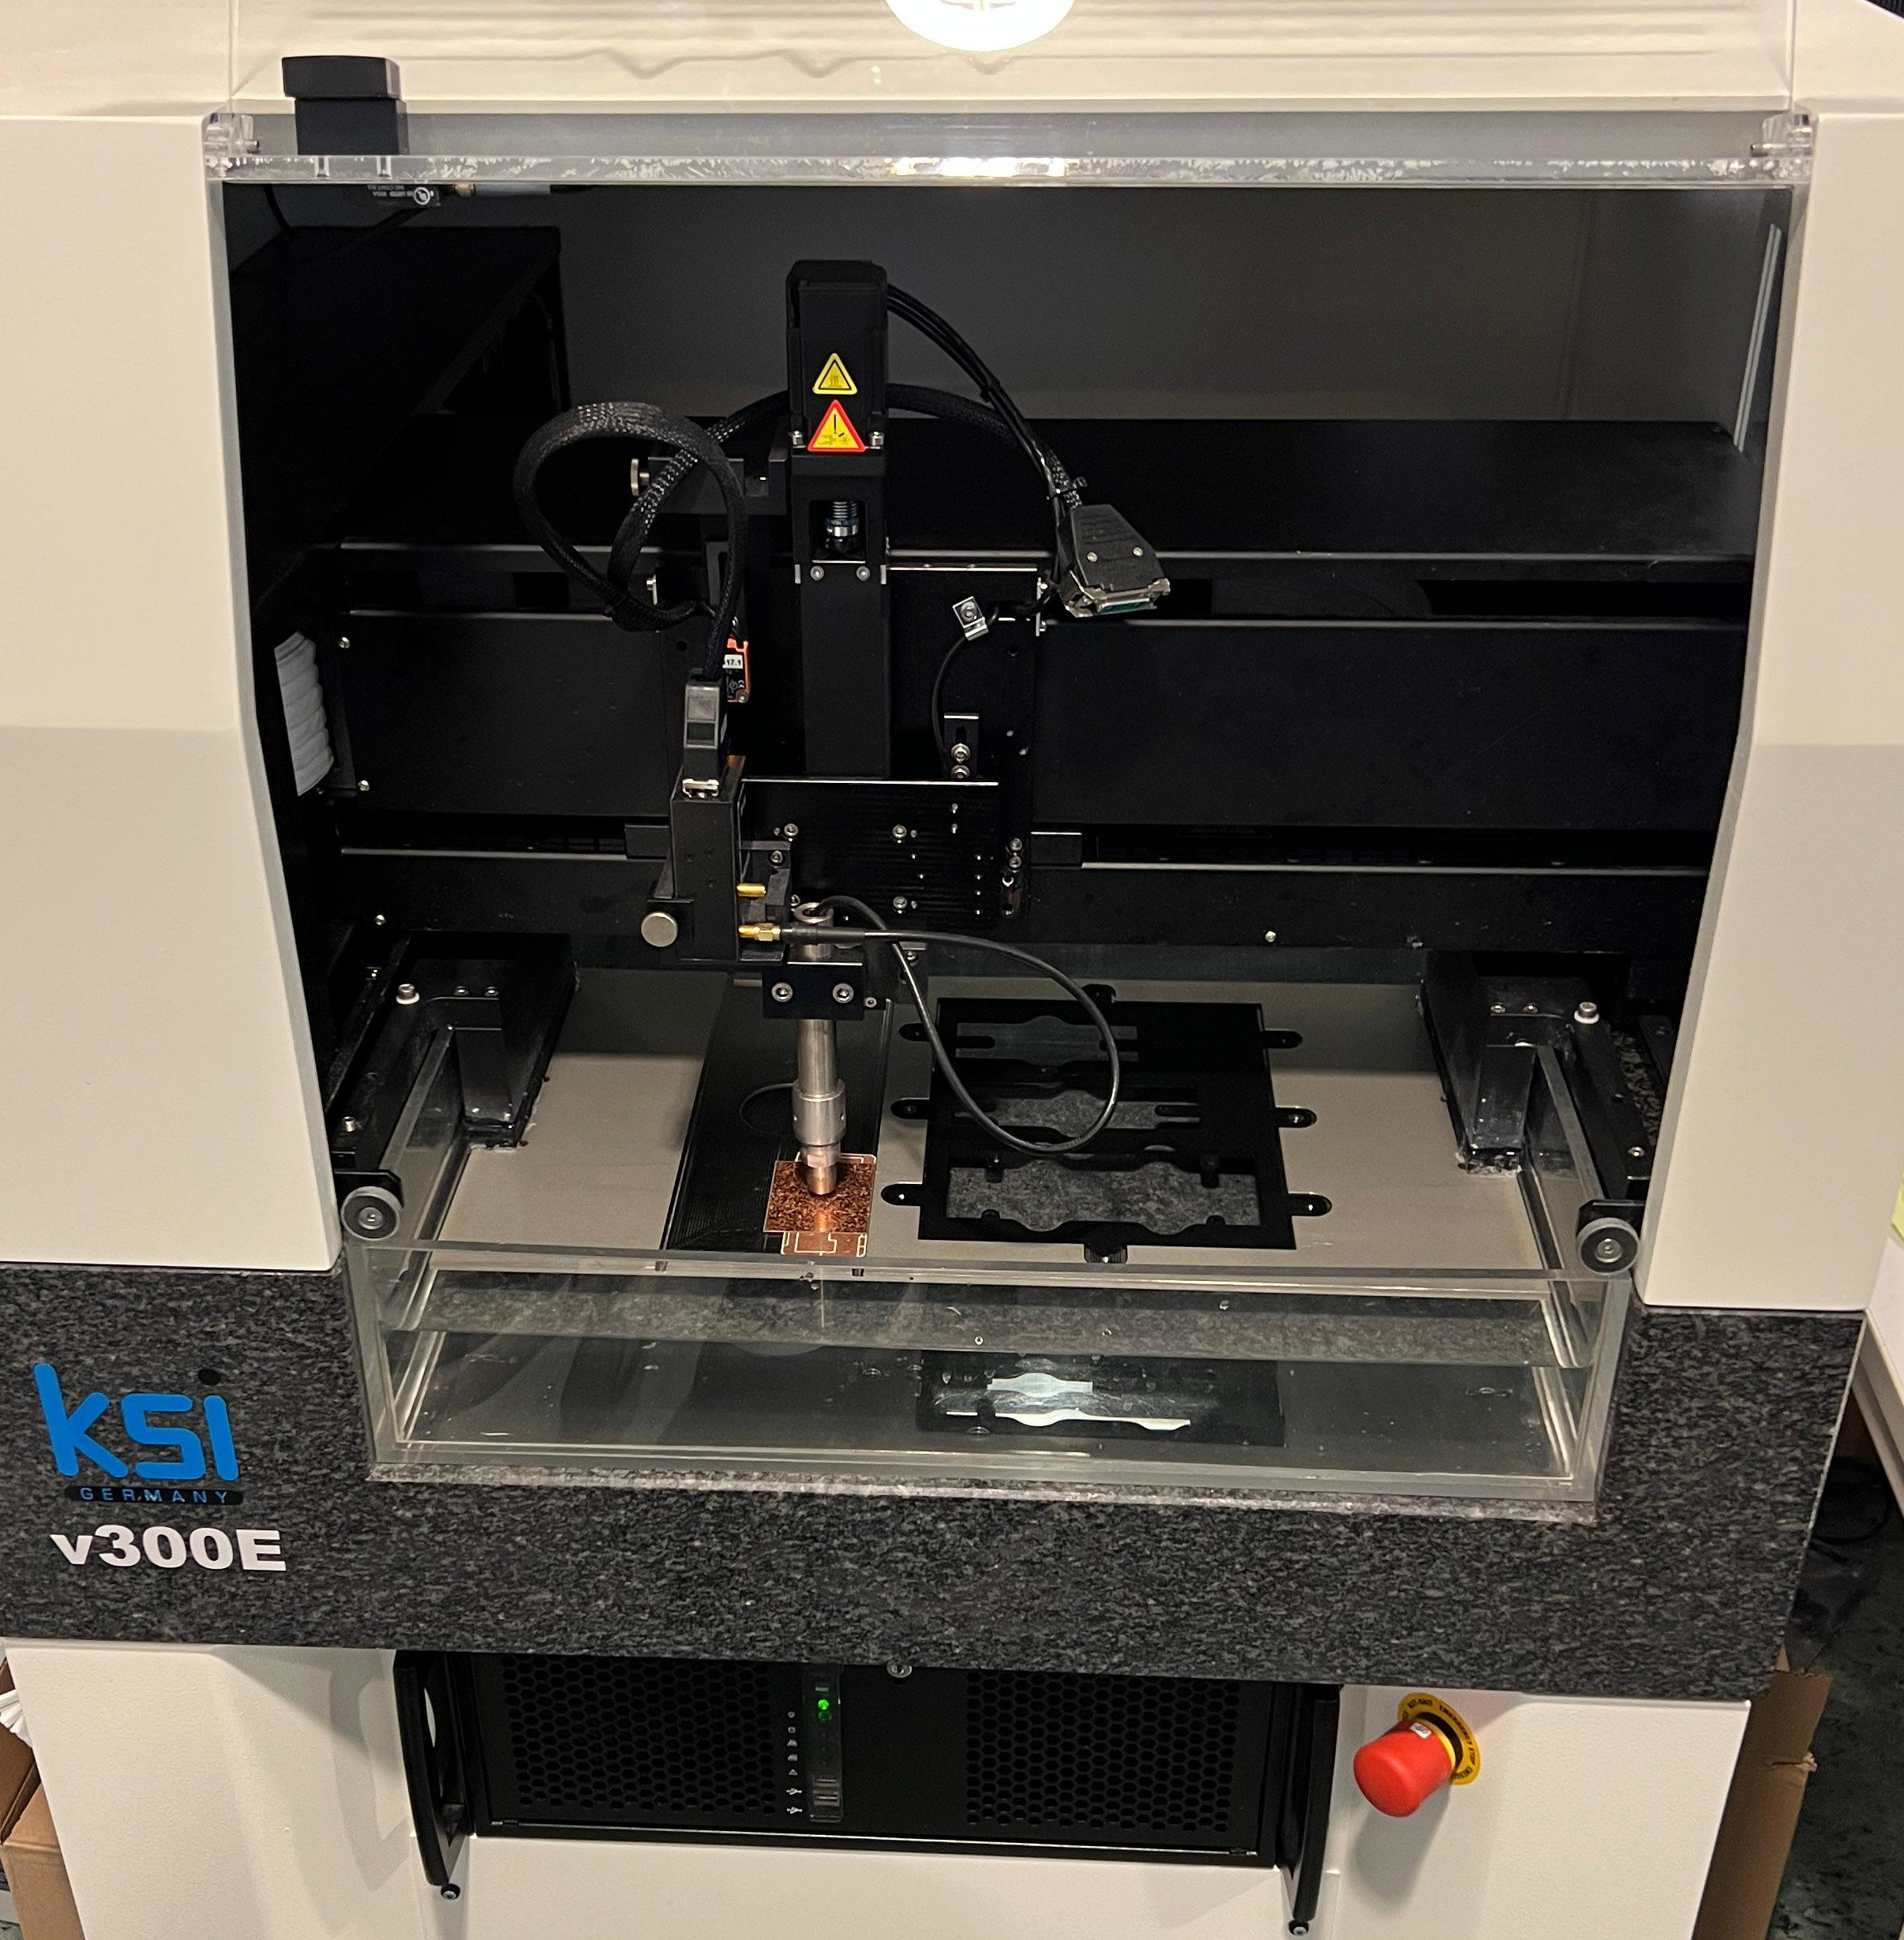
\includegraphics[scale=0.11]{Bilder/ksiv8}
    \caption{KSI v300E Ultraschallmikroskop am Messplatz. Die Probe wird in einem Wasserbad positioniert und mittels eines piezoelektrischen Wandlers im Reflexionsmodus untersucht.}
    \vspace{0.2cm}
    \label{Abb.2: KSI v300E Ultraschallmikroskop am Messplatz. Die Probe wird in einem Wasserbad positioniert und mittels eines piezoelektrischen Wandlers im Reflexionsmodus untersucht. }
\end{figure} 
\vspace{0.2cm}
\begin{figure}[htbp]
    \centering
    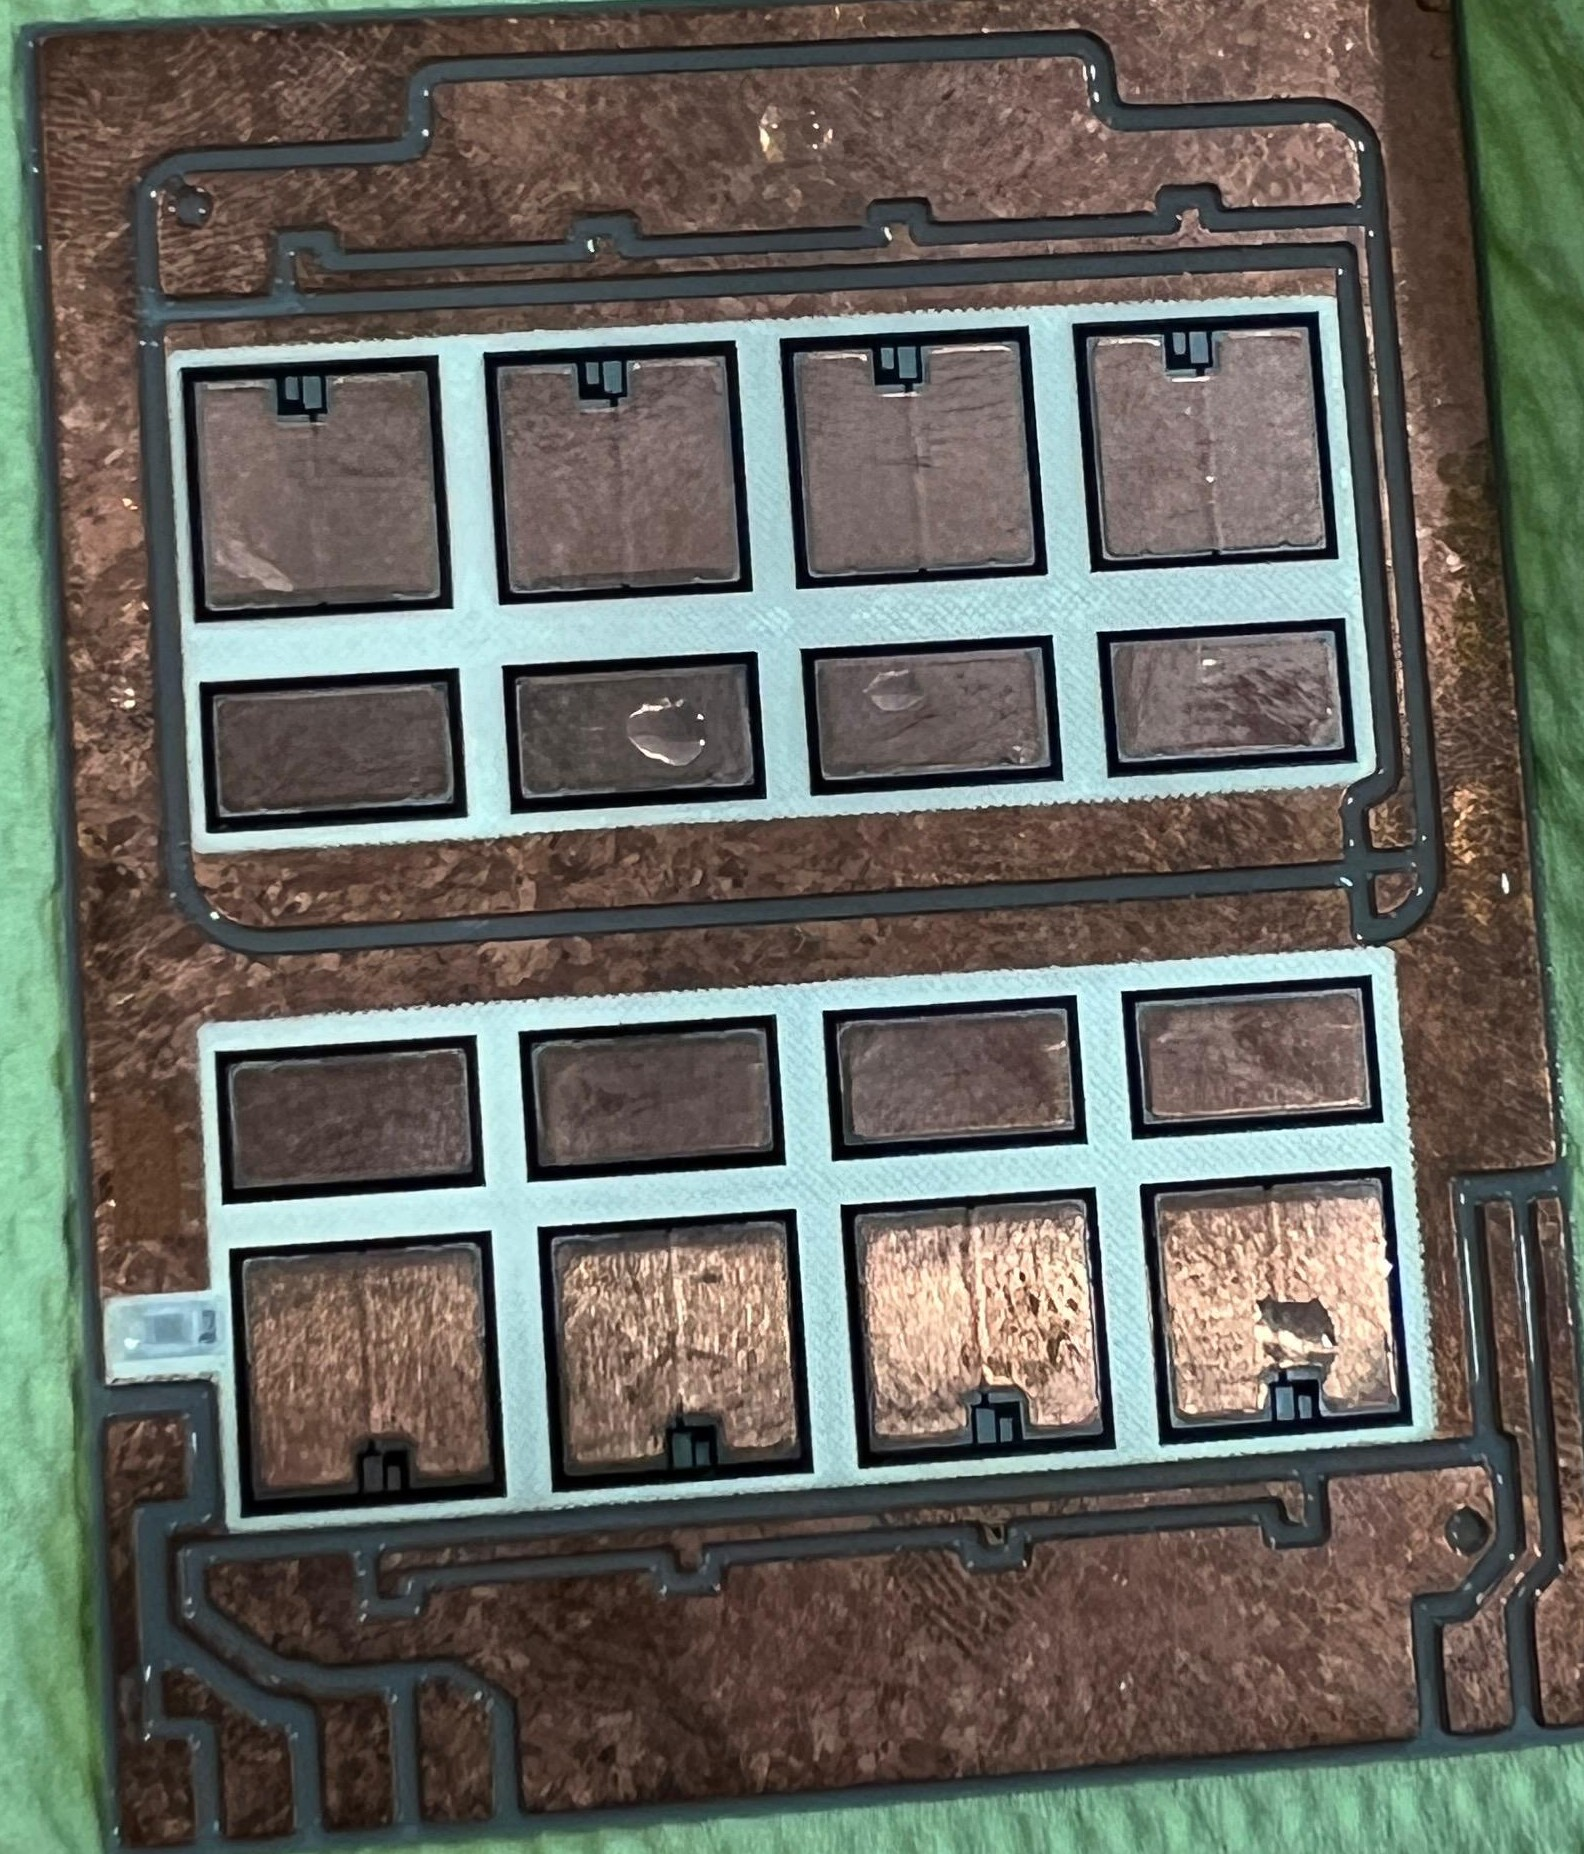
\includegraphics[scale=0.12]{Bilder/probe1}
    \caption{DCB-Leiterplatte mit gesinterten Halbleitern und teilweiser Kontaktierung durch Bonddrähte. Die Probe dient zur Einarbeitung in die Bedienung des akustischen Mikroskops sowie zur Analyse von Materialübergängen.}
    
    \vspace{0.2cm}
    \label{Abb.3: DCB-Leiterplatte mit gesinterten Halbleitern. Die Probe dient zur Einarbeitung in die Bedienung des akustischen Mikroskops sowie zur Analyse von Materialübergängen. }
\end{figure} 
\vspace{0.2cm}
\begin{figure}[htbp]
    \centering
    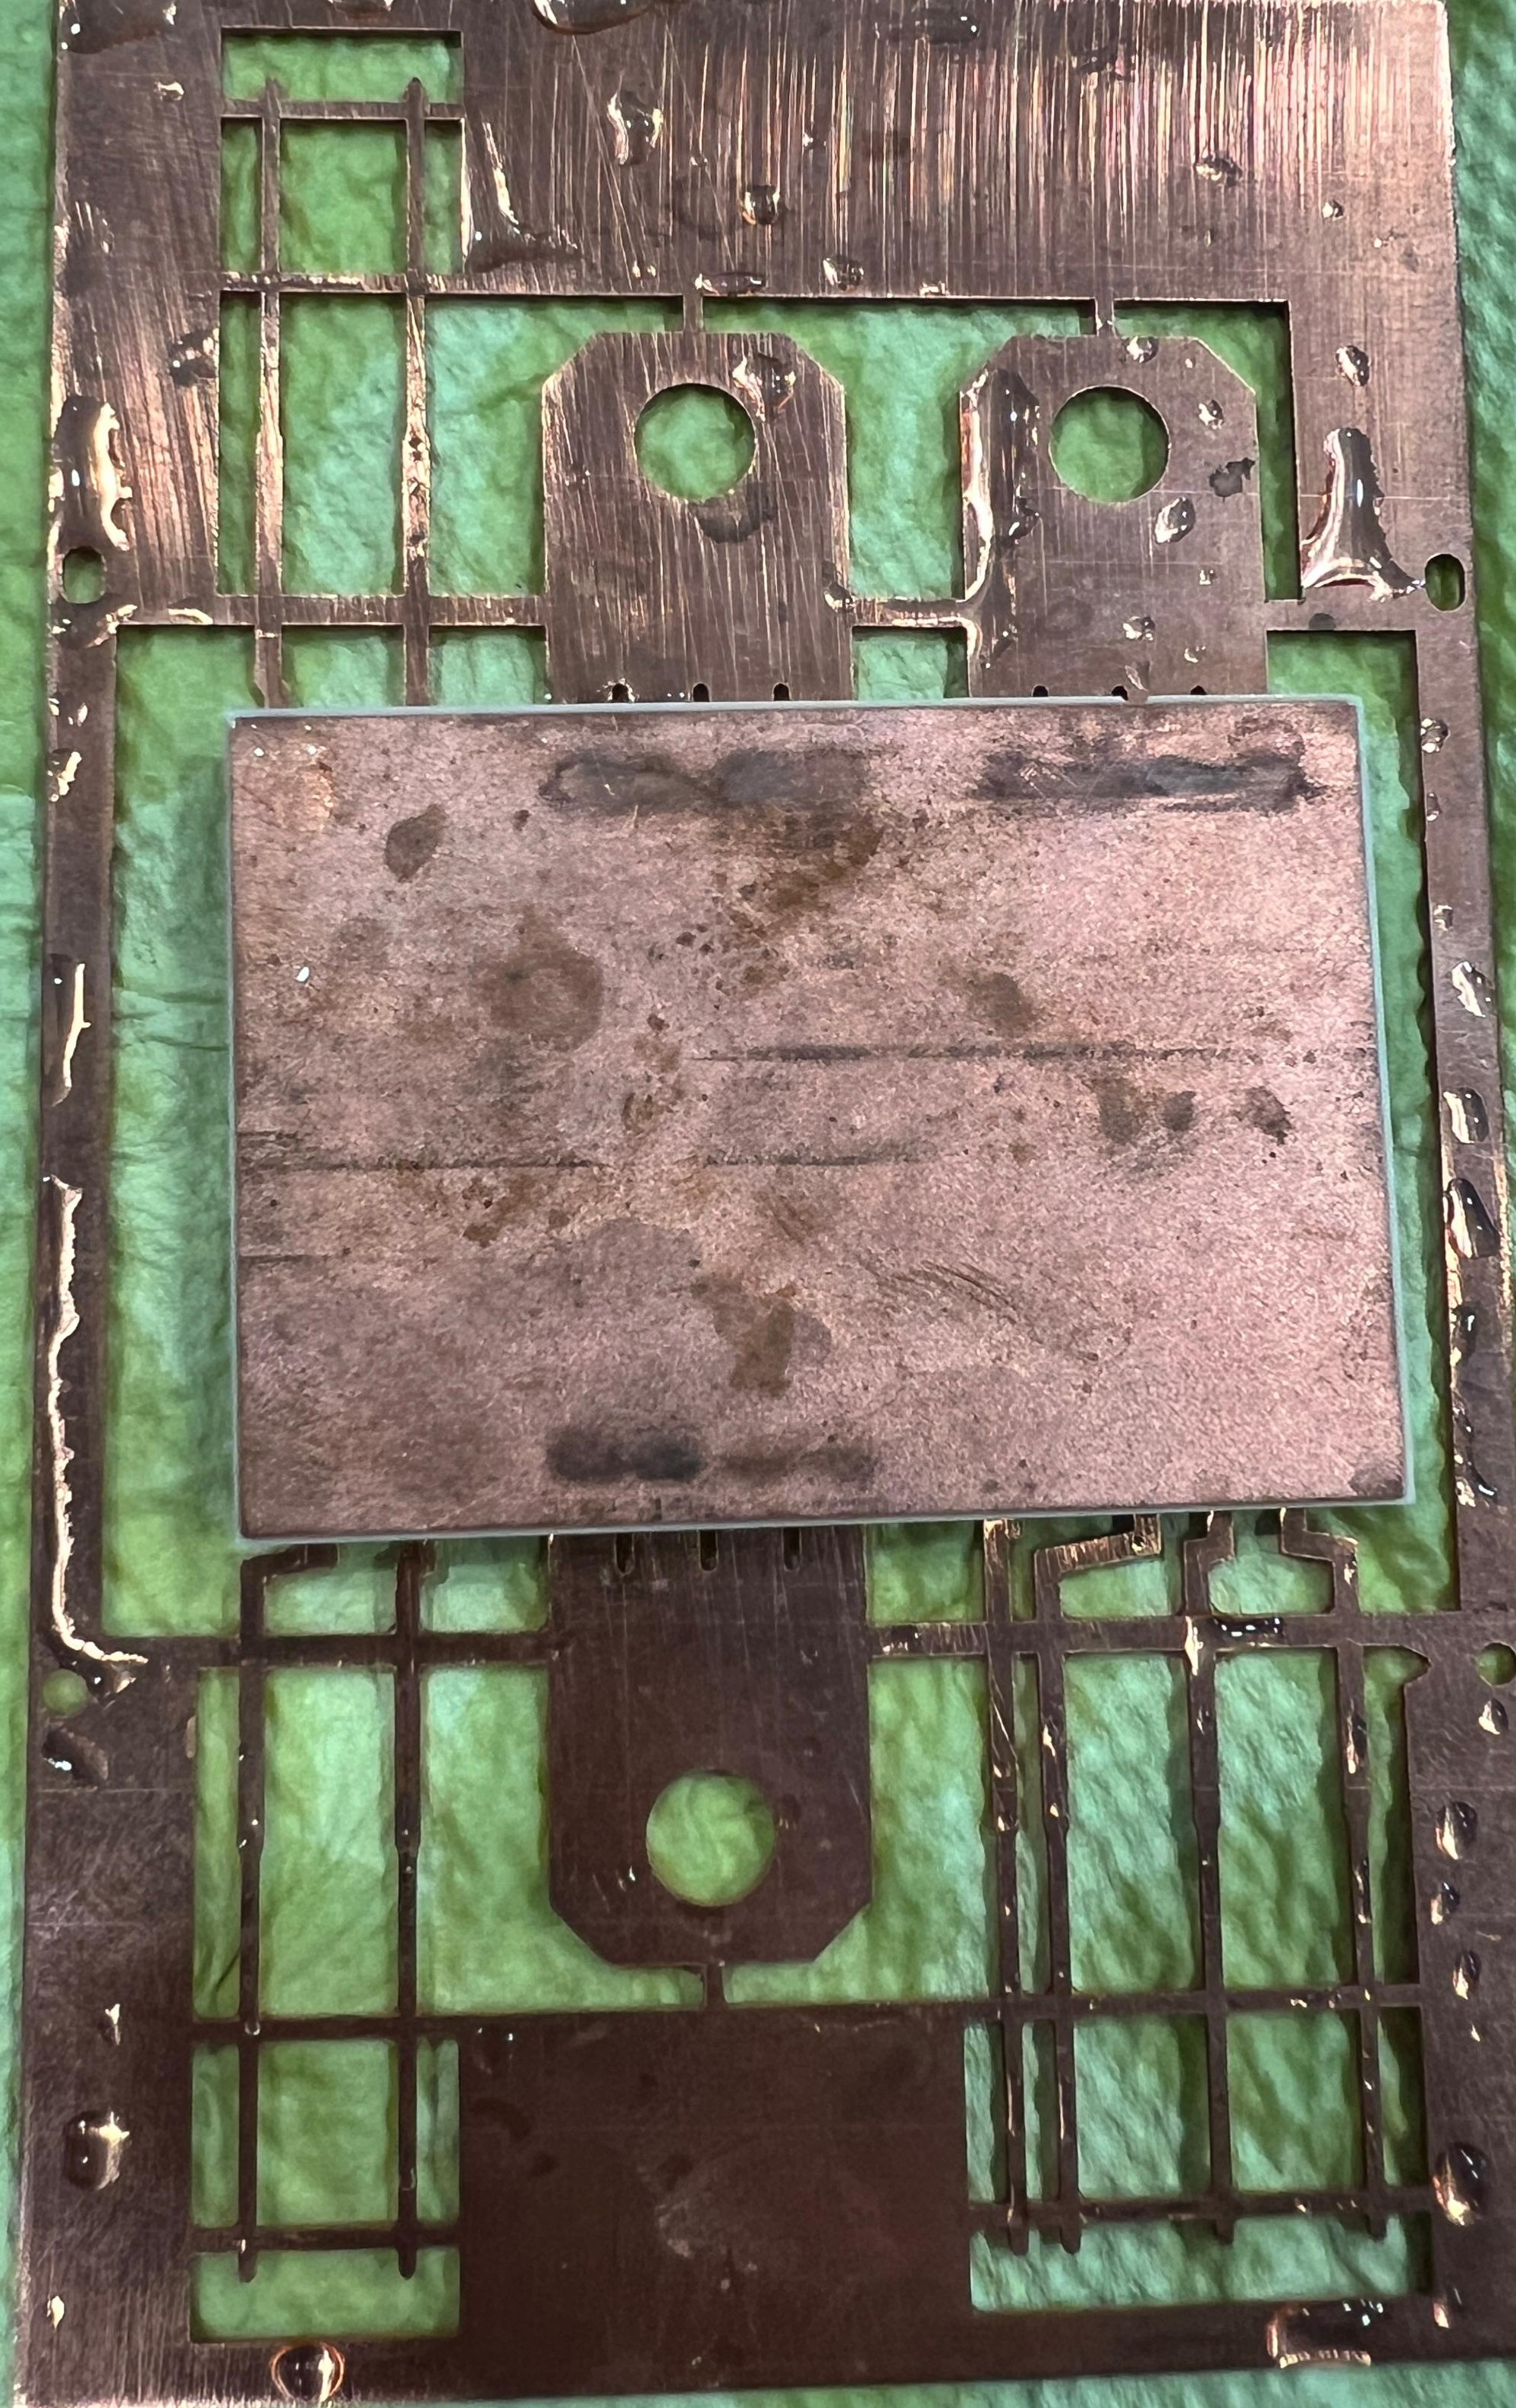
\includegraphics[scale=0.12]{Bilder/probe 2}
    \caption{Keramisches Substrat mit angeschweißtem Kupfer-Leadframe. Die Untersuchung konzentriert sich auf die Qualität der Schweißverbindungen und das Auffinden potenzieller Defekte.}
    \vspace{0.2cm}
    \label{Abb.4: Keramisches Substrat mit angeschweißtem Kupfer-Leadframe. Die Untersuchung konzentriert sich auf die Qualität der Schweißverbindungen und das Auffinden potenzieller Defekte. }
\end{figure} 
\vspace{0.2cm}
\begin{figure}[htbp]
    \centering
    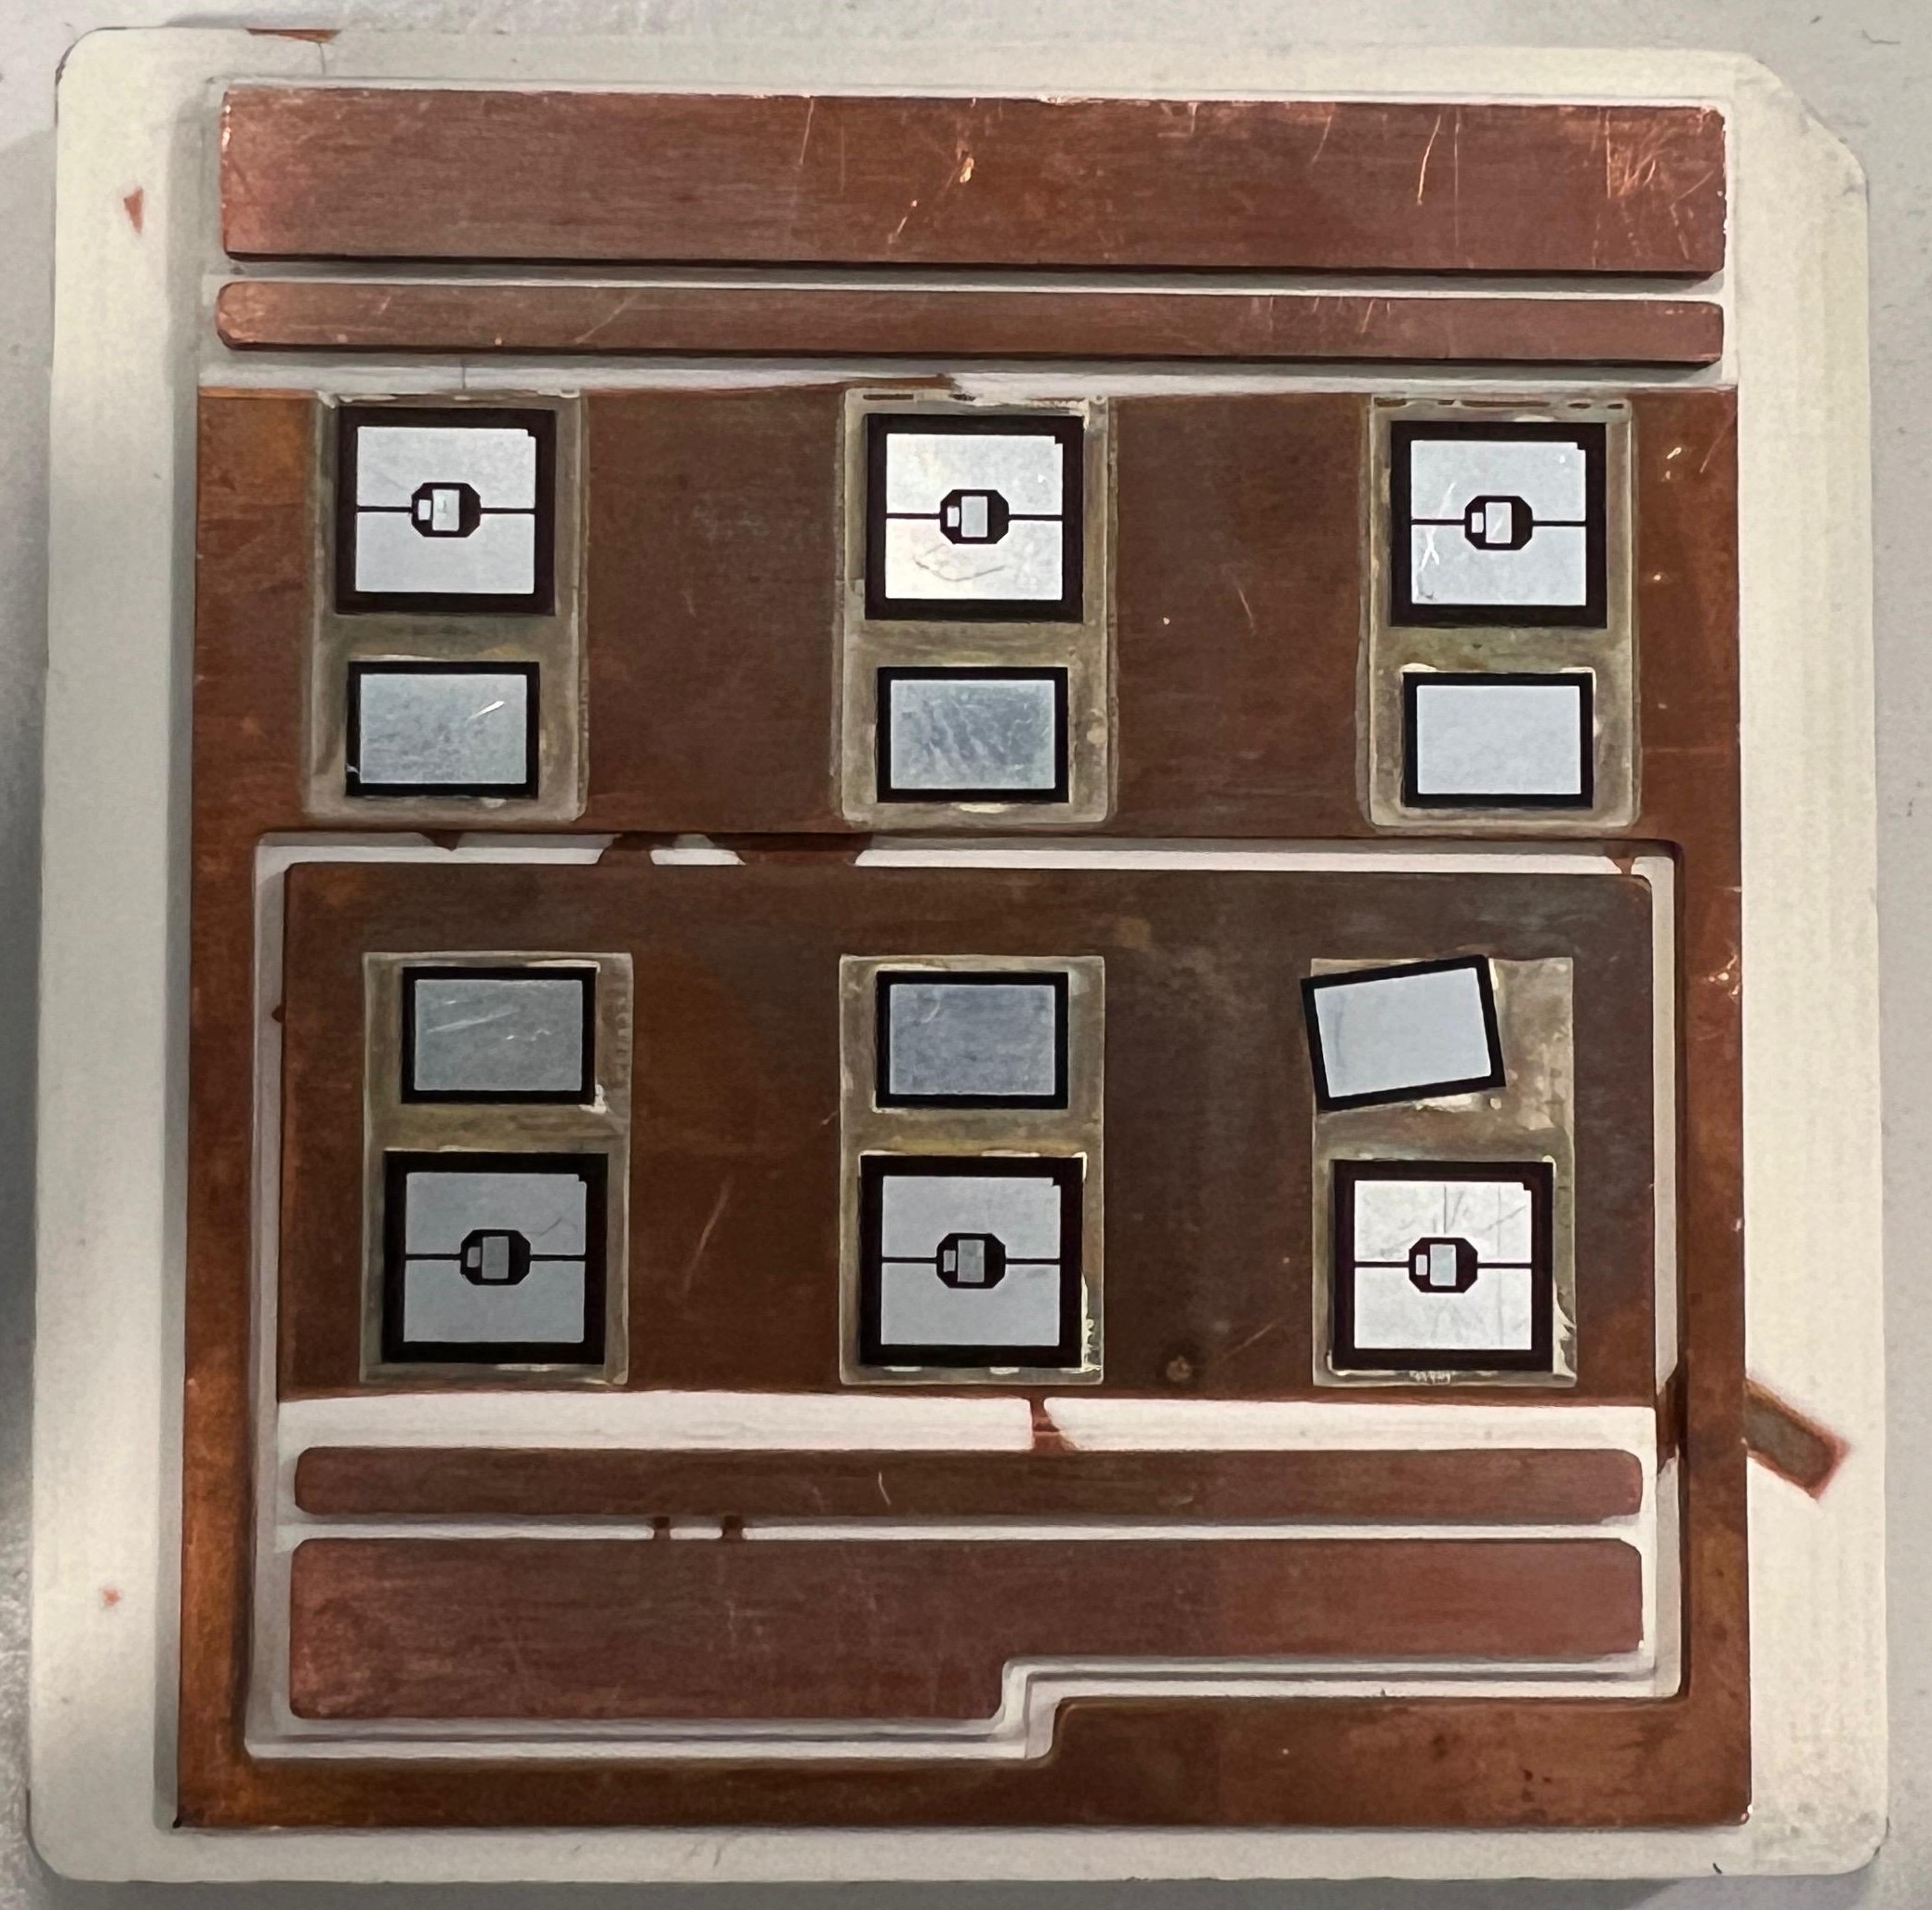
\includegraphics[scale=0.13]{Bilder/probe3}
    \caption{DoL-Leistungselektronikmodul ohne Bonddrähte. Statt keramischer Isolation kommt eine organische Trägerfolie zum Einsatz. Ziel ist die eigenständige Auswahl und Bewertung geeigneter Fokusebenen.}
    \vspace{0.2cm}
    \label{Abb.5: DoL-Leistungselektronikmodul ohne Bonddrähte. Statt keramischer Isolation kommt eine organische Trägerfolie zum Einsatz. Ziel ist die eigenständige Auswahl und Bewertung geeigneter Fokusebenen. }
\end{figure} 
\vspace{0.2cm}